\subsection{Active learning}
Even with the most advance neural network architecture, it is still impossible to achieve a acceptable result without a sufficient amount of labeled data. However, the acquisition of labeled data for new tasks is both challenging and costly. In such case, active learning can be used to lower the cost of annotation without sacrificing. The motivation behind active learning focus on, given a pool of unlabeled data and a limited annotation-budget, there must exist an optimal way to query the best sub-set of it for label, such that sub-set queried by active learning would significantly outperform a random selected sub-set. The problem of active learning in image classification can be formulated as follow. Given  an unlabeled data-set of $X^U$ and a labeled data-set of $X^L$ , the algorithm need to take $k$ samples from $X^U$, query the correspond label from an oracle and add them to $X^L$ in order to minimize the classification error of a model trained on $X^L$.
\subsection{Batch-mode Active learning}
In most active learning research, the queries are selected one at a time, i.e serial. However, such method is sometimes very very inefficient and time-consuming \cite{activelearningbook}. In many cases, there would be multiple annotators working on different labeling workstations at the same time span on a network and the query speed is not fast enough to catch up with the labeling speed. In such cases, active learning method that selecting queries in serial may be inefficient and this has given rise to batch-mode active learning. Batch-mode active learning allow the learner to query instances in groups, which proof to be more effective for parallel labeling or network with long training time. The goal of batch-mode active learning is to select an optimal query set $\mathbf{Q}$ which performance is comparable with serial selecting. Although, it is very challenging since the active learner fails to consider the overlap in information content among the selected instances and for batch. There has been several research studies that address this problem \cite{Discriminativebatchmode} and various of proposed method to combat this \cite{6912976}. For the most part, these approaches has show a better result then random batch sampling, but still not comparable to serial query. \cite{activelearningbook}
\subsection{Active learning in image classification}
Active learning has been applied and achieved a considerable amounts of success in different area of machine learning, from speech recognition to object detection \cite{workshop}. As for image classification, the key idea of active learning revolve around achieve greater accuracy with fewest number of labeled training samples. One of the most common approach is uncertainty base active learning, where the learner select instances based on the classifier uncertainty. However, we can also perform selection base on dissimilarity between instances, i.e distances between data points or by reducing the expected error reduction by simulate the label outcome of each instances. 


\subsection{Uncertainty base active learning}
One of the most basis and simplest method in active learning is to query base on the uncertainty of the classifier. For this method there are 3 main way to determine the selection criteria: Least confidence (LC), margin sampling (MS) \cite{roy2001toward}, and entropy \cite{shannon1948mathematical}. 
\subsubsection{Least confidence selection}
This method query instances one by one by select the unlabeled instances $x_i$ that have lowest score given by the function $max(p(y_j|x_i))$, which is the probability of instance $x_i$ belongs to class $y_j$.
\begin{equation}
    x^{LC}_i =\underset{x \in X^U}{argmin} ( max(p(y_j|x_i)))
\end{equation}
\subsubsection{Margin sampling selection}
This strategy pick the sample with the smallest probability different of the top two class predictions $y_1$ and $y_2$.
\begin{equation}
    x^{MS}_i =\underset{x \in X^U}{argmin} ( (p(y_1|x_i)- p(y_2|x_i)))
\end{equation} 
\subsubsection{Entropy selection}
The selection takes all class label probabilities into consideration to measure uncertainty and select the one with largest class prediction information entropy.
\begin{equation}
    x^{entropy}_i =\underset{x \in X^U}{argmax} (\sum_{j}p(y_j|x_i)log(p(y_j|x_i))
\end{equation} 
\subsection{Deep Bayesian Active Learning}
Deep Bayesian Active Learning(BALD) \citet{GalIG17}, is one of the more sophisticated uncertainty base method of active learning designed for deep CNN. The method make use of the Bayesian equivalent of CNN\citet{gal2015bayesian}, which are CNNs with prior probability distribution placed over a set of model parameters $\omega = {W_1, ... , W_L}$. To achieve this, we applied stochastic regularization techniques such as dropout where dropout can be interpreted as a variational Bayesian approximation. The prediction probabilities of an instance in this case will be:
\begin{equation}
    p(y_j|x_i) = \frac{1}{T} \sum_{t=1}^Tp(y_j|x_i, \hat{\omega}_t)
\end{equation} 
with T is the number of different outcome of the neural network affected by $\hat{\omega{_t}}$ with $\hat{\omega{_t}} \sim q^{*}_\theta(\omega)$ where  $q^{*}_\theta(\omega)$ is the dropout distribution. The selection function of this method can be written as follows:
\begin{equation}
    x^{BALD}_i =\underset{x \in X^U}{argmin} (- log(p(y_j|x_i)) + \frac{1}{T}\sum_{t=1}^Tp(y_j|x_i,\hat{\omega}_t)log(p(y_j|x_i,\hat{\omega}_t)))
\end{equation}
where $p(y_j|x_i, \hat{\omega}_t)$ is the prediction probability of each CNN with different weight parameters affected by dropout.  
\subsection{Deep Bayesian Active Learning}    
\subsection{Cost-effective active learning}
\begin{equation}
    S^{A}_{x} = \begin{bmatrix}
       |5| \\[0.3em]
       \frac{5}{6} \\[0.3em]
       0           
     \end{bmatrix}
\end{equation}
\subsection{Criteria switching active learning}
As previous mentioned, active learning is st 
\begin{figure}[ht]
\begin{center}
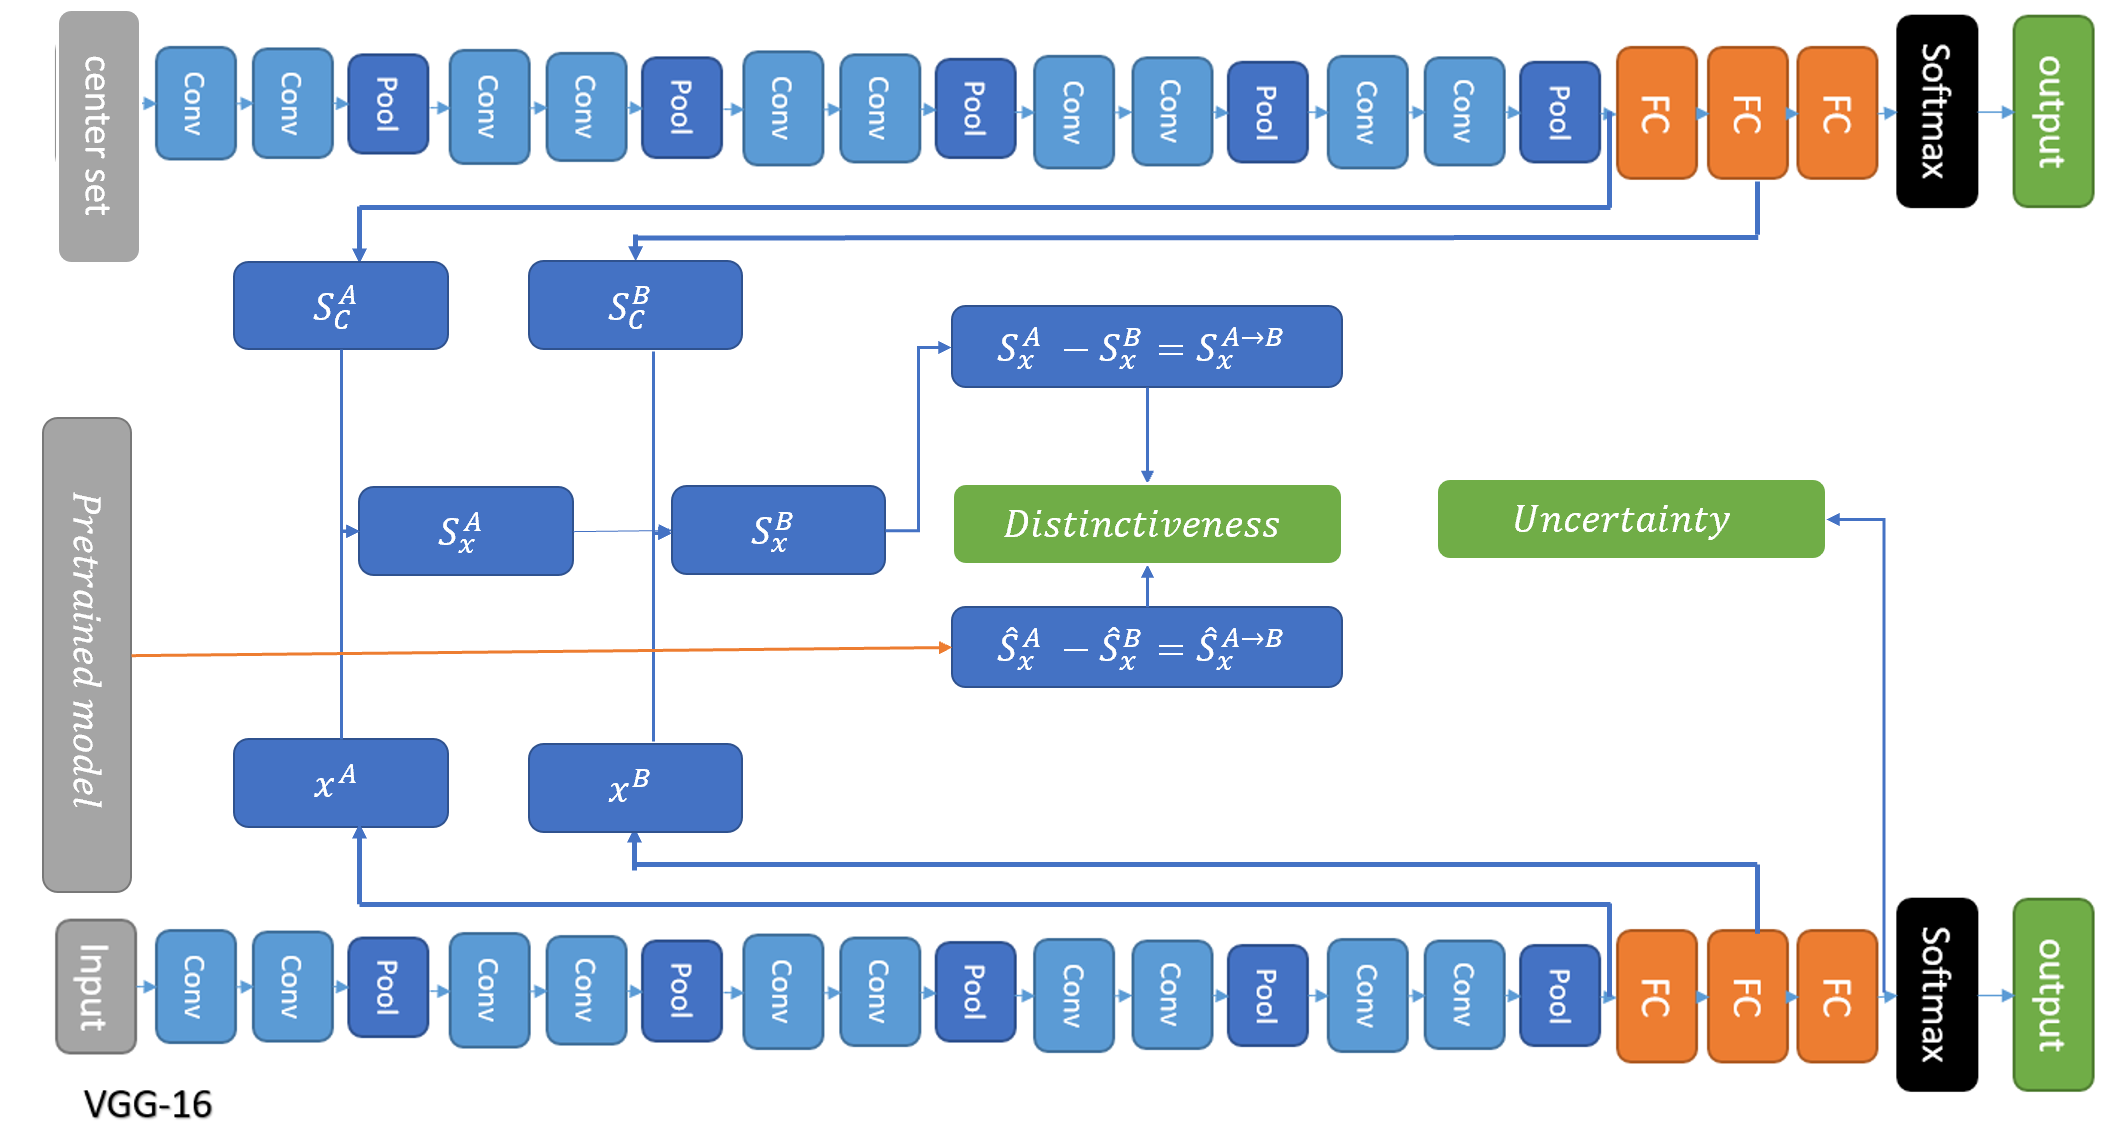
\includegraphics[width=1\columnwidth]{Image/vgg.PNG}
\caption[vgg]{ cost effective }
\label{fig:BoxesAndArrowsAreNice}
\end{center}
\end{figure}
\cite{costeffective}
\cite{costeffective2}